\chapter{Kolmogorov, Cybernetics and the Thermodynamics of Information}
\label{ch:kolmogorov}

\section{Kolmogorov in three roles}

Andrei Kolmogorov is among the mathematicians who appear most often in this book. He gave the axioms of probability in 1933~\cite{kolmogorov1933}, the forward and backward equations of diffusions in 1931~\cite{kolmogorov1931}, the theory of turbulence in 1941~\cite{kolmogorov1941a}, the traveling front of the Fisher equation in 1937~\cite{kolmogorov1937}, the superposition theorem that answered Hilbert's thirteenth problem in 1957~\cite{kolmogorov1957}, the invariant tori of perturbed Hamiltonian systems in 1954~\cite{kolmogorov1954}, and the algorithmic definition of information in 1965~\cite{kolmogorov1965}. He also thought hard about machines that learn. Wiener's \emph{Cybernetics}~\cite{wiener1948} appeared in 1948 and was denounced in the Soviet press as a bourgeois pseudoscience~\cite{gerovitch2002}; within a decade the political climate had changed. In 1961 Kolmogorov gave a lecture, \emph{Automata and Life}, which we read as arguing that there is no principled barrier to the construction of machines whose behavior is as complex as that of living beings, that the question of whether machines can think is a scientific question to be settled by the analysis of what thinking does rather than by definitions, and that the study of living systems and of automata should share a single mathematical language of information and control.

This chapter takes Kolmogorov's view seriously and asks what it means for the inferential sixth problem. If inference is a physical process, carried out by brains, by computers and by the scientific community, then it has a mechanics and a thermodynamics, and both are within the scope of Hilbert's request.

\section{The superposition theorem}

Hilbert's thirteenth problem asked whether the solution of the general equation of degree seven, as a function of its coefficients, can be written as a composition of continuous functions of two variables. A Tschirnhaus transformation reduces the equation to $x^7+ax^3+bx^2+cx+1 = 0$, so that only three parameters $a$, $b$, $c$ remain. Kolmogorov and Arnold, then Kolmogorov's student, answered a much stronger question in 1957~\cite{kolmogorov1957}.

\begin{theorem}[Kolmogorov superposition]
There exist continuous increasing functions $\phi_{q,p}:[0,1]\to\R$, for $q = 0,\dots,2n$ and $p = 1,\dots,n$, such that every continuous $f:[0,1]^n\to\R$ can be written as
\[
f(x_1,\dots,x_n) = \sum_{q=0}^{2n}g_q\Big(\sum_{p=1}^n\phi_{q,p}(x_p)\Big)
\]
for suitable continuous functions $g_q$ of one variable, depending on $f$.
\end{theorem}

The inner functions are universal; only the outer ones depend on $f$. Every continuous function of several variables is therefore a superposition of continuous functions of one variable and addition. We quote the theorem without proof; Braun and Griebel~\cite{braungriebel2009} give a constructive proof. The outer functions are continuous but not unique, and they can vary wildly even when $f$ is smooth~\cite{schmidthieber2021}. Arnold had shown earlier the same year~\cite{arnold1957} that every continuous function of three variables is a superposition of continuous functions of two variables, contradicting the answer Hilbert had expected.

The theorem has a long and somewhat contested history as a justification for neural networks: a network with two hidden layers of univariate nonlinearities can represent any continuous function exactly. The inner functions are rough: they are continuous and increasing, hence differentiable almost everywhere, but their graphs resemble that of the Cantor function~\cite{schmidthieber2021}, so exact representation says little about learnability, and Girosi and Poggio~\cite{girosipoggio1989} declared the theorem irrelevant for neural networks. But the structure, sums of univariate functions composed with univariate functions, is that of generalized additive models, and Kolmogorov Arnold networks~\cite{liu2024kan} with smooth learned univariate pieces are a practical descendant. For the themes of this book the important point is different: Kolmogorov showed that the apparent complexity of a high dimensional function can be reduced, without loss, to a small number of one dimensional operations arranged in the right architecture. The search for such architectures is the search for representations in which inference is easy.

\section{Algorithmic information}

Recall from Chapter~\ref{ch:axioms} the prefix Kolmogorov complexity $K(x)$ of a finite string. It is uncomputable but approximable from above, invariant up to an additive constant, and connected with Shannon entropy by the theorem that for independent samples from a computable law $P$,
\[
\frac1n\E K(X_1,\dots,X_n)\to H(P).
\]
The universal prior $m(x)\approx2^{-K(x)}$ dominates every computable prior, so Bayesian prediction with $m$ incurs total log loss at most $K(P)\log2$ more than prediction with the true $P$. Rissanen's minimum description length principle~\cite{rissanen1978} and its refinements are practical versions: choose the model that gives the shortest two part code for the data, the description of the model plus the description of the data given the model. For regular parametric families with a $d$ dimensional parameter $\theta$ the two part code length is
\[
-\log p(x_{1:n}\mid\hat\theta)+\frac d2\log n+O(1),
\]
which is half the Bayesian information criterion. The refined code length, the stochastic complexity of Rissanen~\cite{rissanen1996}, is
\[
-\log p(x_{1:n}\mid\hat\theta)+\frac d2\log\frac n{2\pi}+\log\int\sqrt{\det J(\theta)}\dd\theta+o(1),
\]
where $J$ is the Fisher information matrix and the integral runs over a compact parameter set. It agrees to $o(1)$ with the negative log marginal likelihood under Jeffreys' prior. Occam's razor, Bayesian model selection and compression are one principle.

\section{Maxwell's demon}

In a letter to Tait in 1867, and in the \emph{Theory of Heat} of 1871~\cite{maxwell1871}, Maxwell imagined a being who controls a trapdoor between two chambers of gas and lets only fast molecules pass one way and slow ones the other, creating a temperature difference without work, in apparent violation of the second law. For sixty years the demon resisted exorcism. Smoluchowski argued in 1912~\cite{smoluchowski1912} that thermal fluctuations of any mechanical trapdoor would defeat it. The decisive analysis began with Szilard in 1929~\cite{szilard1929}.

Szilard reduced the demon to its information theoretic core: a single molecule in a box of volume $V$ in contact with a heat bath at temperature $T$. A partition is inserted in the middle, the demon observes which half the molecule is in, attaches a piston on the empty side, and lets the molecule push the piston isothermally back to volume $V$. The work extracted is
\[
W = \int_{V/2}^{V}\frac{k_BT}{v}\dd v = k_BT\log2.
\]
One bit of information about the molecule's position converts into $k_BT\log2$ of work from a single heat bath. If the demon could repeat the cycle indefinitely, the second law would fail; therefore, Szilard argued, acquiring or handling the bit must cost at least $k_BT\log2$ of dissipation.

Szilard located the cost in the measurement. Landauer in 1961~\cite{landauer1961} located it elsewhere: logically irreversible operations, such as erasing a bit of unknown value to reset a memory, must dissipate at least $k_BT\log2$ per bit, because they compress the phase space of the memory and must export the corresponding entropy to the environment. Bennett in 1982~\cite{bennett1982} completed the argument by showing that measurement can be done reversibly, so the demon's unavoidable cost is the erasure of its memory at the end of each cycle, which exactly compensates the work extracted. B\'erut and coauthors confirmed Landauer's bound experimentally in 2012~\cite{berut2012} with a colloidal particle in a double well potential, observing that the mean dissipated heat approaches $k_BT\log2$ in the limit of slow erasure.

\begin{theorem}[Landauer bound, information theoretic form]\label{thm:landauer}
Let a memory with finitely many states of equal energy and a heat bath at temperature $T$ be initially independent, the memory having the distribution $p$ and the bath being in its Gibbs state at temperature $T$. Let the memory and the bath then evolve together under reversible dynamics, Hamiltonian or unitary, possibly driven by a protocol fixed in advance, until the memory has the distribution $q$, and let $Q$ be the energy gained by the bath. Then
\[
\E Q\geq k_BT\big(H(p)-H(q)\big)\log2,
\]
with entropies in bits. In particular erasing a uniformly random bit, $H(p) = 1$, $H(q) = 0$, dissipates at least $k_BT\log2$.
\end{theorem}

\begin{proof}
Measure entropy in units of $k_B$. The memory then has entropy $H(p)\log2$ when its distribution is $p$, and we write $S(\pi)$ for the entropy of the bath in the state $\pi$. Reversible dynamics conserve the entropy of the joint state. Initially the joint state is a product, with entropy $H(p)\log2+S(\pi_0)$, where $\pi_0\propto e^{-\mathcal H_B/k_BT}$ is the Gibbs state of the bath with Hamiltonian $\mathcal H_B$. Finally the entropy of the joint state is at most the sum $H(q)\log2+S(\pi_1)$ of the entropies of its marginals, where $\pi_1$ is the final state of the bath. Hence $S(\pi_1)-S(\pi_0)\geq(H(p)-H(q))\log2$. On the other hand, writing out $\KL(\pi_1\|\pi_0)\geq0$ for the Gibbs state $\pi_0$ gives $S(\pi_1)-S(\pi_0)\leq(\E_{\pi_1}\mathcal H_B-\E_{\pi_0}\mathcal H_B)/k_BT = \E Q/k_BT$. The two bounds together give the claim.
\end{proof}

The bound is the exchange rate between information and energy, and it is the thermodynamic content of the inferential sixth problem.

\section{Kelly: information as growth}

In 1956 John Kelly, at Bell Laboratories, gave Shannon's information rate an economic interpretation~\cite{kelly1956}. A gambler bets repeatedly on a binary event of probability $p>\frac12$ at even odds, wagering a fraction $f$ of capital on the favored outcome. The capital after $n$ bets is $B_n = B_0\prod_{i=1}^n(1+fs_i)$, with $s_i = +1$ if bet $i$ is won and $s_i = -1$ if it is lost, and its exponential growth rate is
\[
G(f) = \lim_n\frac1n\log_2\frac{B_n}{B_0} = p\log_2(1+f)+(1-p)\log_2(1-f).
\]

\begin{theorem}[Kelly]\label{thm:kelly}
$G$ is maximized at $f^* = 2p-1$, and $G(f^*) = 1-H(p)$ bits per bet, where $H(p) = -p\log_2p-(1-p)\log_2(1-p)$. More generally, for a horse race with win probabilities $p_i$ and odds $o_i$, meaning that a unit bet on horse $i$ returns $o_i$ if it wins, with $\sum1/o_i = 1$, betting the fraction $b_i$ of wealth on horse $i$ gives growth rate
\[
G(b) = \sum_ip_i\log_2(b_io_i) = \KL(p\,\|\,r)-\KL(p\,\|\,b),\qquad r_i = 1/o_i,
\]
maximized by proportional betting $b = p$.
\end{theorem}

\begin{proof}
The identity follows from $\log_2(b_io_i) = \log_2(p_i/r_i)-\log_2(p_i/b_i)$. Since $\KL(p\|b)\geq0$ with equality iff $b = p$, proportional betting is optimal. For the binary case with even odds, $r = (\frac12,\frac12)$ and $\KL(p\|r) = 1-H(p)$; betting $b = (p,1-p)$ of wealth on the two outcomes is equivalent to a net fraction $f = 2p-1$ on the favored one.
\end{proof}

Figure~\ref{fig:kelly} shows the growth curve for $p = 0.6$. The maximal growth $1-H(0.6)\approx0.029$ bits per bet is exactly the information an observer has about the outcome beyond a fair coin. Kelly's theorem is the economic twin of Szilard's engine: Szilard converts a bit of information into $k_BT\log2$ of work, and Kelly converts a bit of information into a doubling of capital. In both, the conversion rate is set by relative entropy, and in both, overestimating one's information is costly: betting more than $f^*$ reduces growth, and betting $2f^*$ gives a slightly negative growth rate, of order $(2p-1)^4$, where the maximum is of order $(2p-1)^2$. Fractional Kelly strategies trade growth for reduced variance, and in our analysis of a well known trading record, \emph{Twenty Two Bits}~\cite{polsonsokolov2026twentytwobits}, we use this calculus to translate realized returns into the implied information rate of the strategy.

\begin{figure}[t]
\centering
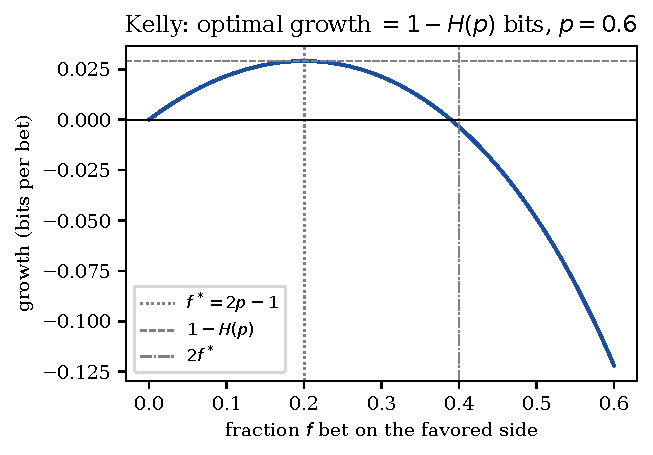
\includegraphics[width=0.92\textwidth]{kelly}
\caption{Kelly growth rate in bits per bet for $p=0.6$ at even odds. The maximum at $f^*=2p-1$ (dotted vertical line) equals $1-H(p)$ (dashed horizontal line). The curve crosses zero at $f\approx0.389$, just below $2f^*=0.4$ (dash dotted vertical line), where the growth is slightly negative.}
\label{fig:kelly}
\end{figure}

\section{Learning systems as thermodynamic engines}

A learning system observes data, updates an internal model, and acts. The data processing inequality states that for a Markov chain $\Theta\to Y\to Z$, $I(\Theta;Z)\leq I(\Theta;Y)$: no processing of the data can increase its information about the truth. Consider a model that is retrained repeatedly on its own outputs.

\begin{proposition}[Recursive self learning]\label{prop:recursive_self_learning}%
Let $\Theta$ be a target and let $M_0$ be a model with $I(\Theta;M_0) = i_0$. Suppose $M_{k+1}$ is computed from $M_k$ and from fresh randomness independent of $\Theta$. Then $I(\Theta;M_k)\leq i_0$ for all $k$. If at each round the update also uses the output of a verifier $V_k$ that depends on $\Theta$ through a channel of capacity $C$ bits per round, so that $I(\Theta;V_k\mid M_k)\leq C$, then $I(\Theta;M_k)\leq i_0+kC$.
\end{proposition}

\begin{proof}
In the first case $\Theta\to M_k\to M_{k+1}$ is a Markov chain and the data processing inequality applies. In the second, by the chain rule, $I(\Theta;M_{k+1})\leq I(\Theta;M_k,V_k)\leq I(\Theta;M_k)+I(\Theta;V_k\mid M_k)\leq I(\Theta;M_k)+C$.
\end{proof}

The proposition is simple, but it sets the terms of debates about systems that improve by self play or by training on synthetic data. AlphaZero~\cite{silver2018} is an analogy for the second clause rather than an instance of it. The rules of chess are a perfect verifier, every game ends in a win, draw or loss determined by the rules, and self play converts computation into play of superhuman strength. In the analogy the unknown $\Theta$ is the value of the positions, and each game returns a result that carries at most $\log_23$ bits about it. The analogy is imperfect, because the value of a position is a deterministic consequence of rules that the learner already has: what self play adds is computation on known rules, which is logical rather than statistical information, and the bound $i_0+kC$ does not describe it as stated. In our paper on AI assisted research~\cite{polsonsokolov2026air} we argue that mathematics has the same structure, since proofs can be checked, and that a research program in which a model proposes and a verifier, human or formal, checks behaves like a digital twin of self play. The present book, drafted with extensive machine assistance and reviewed by its authors, is a small instance.

Each round of learning that overwrites a model's parameters removes entropy from the memory that holds them, and by Theorem~\ref{thm:landauer} the minimum dissipation is $k_BT\log2$ times the entropy removed, measured in bits. Overwriting a value that is known in advance removes no entropy and costs nothing in principle. The information gained per round is at most $C$ bits. The thermodynamic efficiency of learning is therefore bounded by the ratio of verified bits gained to bits of entropy removed, and a learning system that removes far more entropy than it learns, as all present digital systems do, operates far from the Landauer limit. A power budget $P$ pays for the removal of at most $P/(k_BT\log2)$ bits of entropy per second, which for the brain's twenty watts is the ceiling discussed in Chapter~\ref{ch:filters}.

\section{Cybernetics revisited}

Wiener defined cybernetics as the science of control and communication in the animal and the machine. Its central notions, feedback, information and homeostasis, were mathematized in the two decades that followed: feedback by the control theory of Pontryagin and Kalman, information by Shannon and Kolmogorov, homeostasis by the stability theory of dynamical systems. What was missing was a theory of learning that was at once statistical, computational and physical. The chapters of Part~\ref{part:statmech} supply pieces of one. Hilbert asked for the axioms of physics; Kolmogorov's lecture can be read as a request for the physics of thought; the two requests meet in the theory of Bayesian inference as a physical process.

\section{Fluctuation theorems}

Landauer's bound (Theorem~\ref{thm:landauer}) is an inequality on average. Its refinements are equalities about fluctuations. Consider a system in equilibrium at inverse temperature $\beta = 1/k_BT$ with Hamiltonian $\mathcal H_{\lambda_0}$, driven by changing a control parameter from $\lambda_0$ to $\lambda_1$ over a finite time, and let $W$ be the work performed along a trajectory.

\begin{theorem}[Jarzynski]
Under Hamiltonian dynamics, or under any Markov dynamics that preserves the instantaneous Gibbs measure for each fixed value of the control,
\[
\E\big[e^{-\beta W}\big] = e^{-\beta\Delta F},\qquad\Delta F = -\beta^{-1}\log\frac{Z_{\lambda_1}}{Z_{\lambda_0}}.
\]
\end{theorem}

\begin{proof}[Proof for Hamiltonian dynamics]
For an isolated system the work is $W = \mathcal H_{\lambda_1}(\Phi(x))-\mathcal H_{\lambda_0}(x)$, where $\Phi$ is the volume preserving flow map. Then
\[
\begin{aligned}\E e^{-\beta W} &= \int\frac{e^{-\beta\mathcal H_{\lambda_0}(x)}}{Z_{\lambda_0}}e^{-\beta(\mathcal H_{\lambda_1}(\Phi(x))-\mathcal H_{\lambda_0}(x))}\dd x\\ &= \frac{1}{Z_{\lambda_0}}\int e^{-\beta\mathcal H_{\lambda_1}(\Phi(x))}\dd x = \frac{Z_{\lambda_1}}{Z_{\lambda_0}},\end{aligned}
\]
by Liouville's theorem.
\end{proof}

\begin{proof}[Proof for Markov dynamics in discrete time]
Let the control take the values $\mu_0 = \lambda_0,\mu_1,\dots,\mu_N = \lambda_1$ in turn. At step $k$ the control moves from $\mu_{k-1}$ to $\mu_k$ with the state $x_{k-1}$ held fixed, which costs the work $w_k(x_{k-1})$ with $w_k(x) = \mathcal H_{\mu_k}(x)-\mathcal H_{\mu_{k-1}}(x)$, and then the state moves to $x_k$ by a Markov kernel $K_{\mu_k}$ that leaves the Gibbs density $\pi_{\mu_k} = e^{-\beta\mathcal H_{\mu_k}}/Z_{\mu_k}$ invariant. The total work is $W = \sum_{k=1}^Nw_k(x_{k-1})$. Since $\pi_{\mu_{k-1}}(x)e^{-\beta w_k(x)} = (Z_{\mu_k}/Z_{\mu_{k-1}})\pi_{\mu_k}(x)$, integrating out $x_0,x_1,\dots$ in turn and using $\int\pi_{\mu_k}(x)K_{\mu_k}(x,y)\dd x = \pi_{\mu_k}(y)$ at each step gives $\E e^{-\beta W} = \prod_{k=1}^NZ_{\mu_k}/Z_{\mu_{k-1}} = Z_{\lambda_1}/Z_{\lambda_0}$.
\end{proof}

The equality is due to Jarzynski~\cite{jarzynski1997}. For Markov dynamics see Jarzynski~\cite{jarzynski1997master}, who works with a master equation, and Crooks~\cite{crooks2000}, who works in discrete time as above.

Jensen's inequality gives $\E W\geq\Delta F$, the second law, as a consequence. The equality is a change of measure identity: it is importance sampling, with the nonequilibrium trajectory as proposal and the target equilibrium as goal, and it is the physical form of the annealed importance sampling algorithm that Neal introduced independently in 2001~\cite{neal2001}, and of the sequential Monte Carlo samplers of Del Moral, Doucet and Jasra~\cite{delmoral2006}. Crooks' theorem~\cite{crooks1999}, which we quote without proof, refines it to a statement about the ratio of the work density $p_F(W)$ of the protocol to the work density $p_R(-W)$ of the time reversed protocol started in equilibrium at $\lambda_1$, $p_F(W)/p_R(-W) = e^{\beta(W-\Delta F)}$, which is a likelihood ratio between time reversed path measures.

Sagawa and Ueda~\cite{sagawaueda2010} extended the second law to systems with measurement and feedback, and we quote their inequality without proof. If a measurement yields mutual information $I$, in nats, between the system and the memory, and the protocol is chosen as a function of the outcome, then
\[
\E W\geq\Delta F-\beta^{-1}I,
\]
so that information can be converted into work at the rate $k_BT$ per nat, exactly Szilard's rate, and a corresponding cost must be paid when the memory is reset. The generalized second law is the thermodynamic counterpart of the data processing inequality: information is a resource, measured in the same units as free energy, and it can be spent but not created.

\section{Rate distortion and the cost of approximate inference}

Shannon's rate distortion theory asks for the minimal number of bits per symbol needed to describe a source $X$ to within expected distortion $D$:
\[
R(D) = \min_{p(\hat x\mid x):\,\E d(X,\hat X)\leq D}I(X;\hat X).
\]
For a Gaussian source with variance $\sigma^2$ and squared error distortion, $R(D) = \frac12\log_2(\sigma^2/D)$ for $D<\sigma^2$, as in Cover and Thomas~\cite{covertomas}. The minimizing channel is a Gaussian posterior: the optimal reconstruction is the posterior mean under a Gaussian prior and observation model. Rate distortion is therefore Bayesian inference read backwards.

Combined with Landauer's principle, rate distortion theory gives a thermodynamic floor for storing approximations. Let $X_1,\dots,X_n$ be independent copies of the source, and let a memory with finitely many states hold reconstructions $\hat X_1,\dots,\hat X_n$ with average distortion at most $D$. Then $H(\hat X_{1:n})\geq I(X_{1:n};\hat X_{1:n})\geq nR(D)$, which is the converse half of the rate distortion theorem, and by Theorem~\ref{thm:landauer} resetting the memory dissipates at least $nR(D)\,k_BT\log2$ on average. For inference, the source is the unknown quantity and the reconstruction is the stored estimate of it.

Blahut's algorithm~\cite{blahut1972} for computing $R(D)$, a counterpart of Arimoto's algorithm for the capacity of a channel~\cite{arimoto1972}, is an alternating minimization of relative entropy of the same type as Sinkhorn's algorithm of Chapter~\ref{ch:gbc}, with the distortion playing the role of the transport cost and the Lagrange multiplier the role of the inverse entropic regularization. It fixes only the marginal of the source, whereas Sinkhorn's algorithm fixes both marginals.

\section*{Exercises}
\begin{enumerate}
\item Compute the Kelly fraction and the optimal growth rate for a bet that returns $o$ on a unit stake if it is won, the convention of Theorem~\ref{thm:kelly}, with win probability $p$ and $po>1$. Even odds are $o = 2$.
\item Show that betting $2f^*$ in the even odds Kelly problem gives growth $-\frac{4}{3\ln2}(2p-1)^4+O\big((2p-1)^6\big)$ bits per bet, which is negative, whereas the growth at $f^*$ is of order $(2p-1)^2$.
\item Prove the data processing inequality from the chain rule for mutual information.
\item Deduce $\E W\geq\Delta F$ from Jarzynski's equality, and show that $\P(W\leq\Delta F-\varepsilon)\leq e^{-\beta\varepsilon}$.
\item Compute $R(D)$ for a Bernoulli$(p)$ source with Hamming distortion.
\end{enumerate}


\section*{Notes}

Our paper with Alec Litowitz~\cite{litowitz2026} follows the line from Shannon's theory of communication to Kolmogorov's theory of complexity. Leff and Rex's anthology \emph{Maxwell's Demon}~\cite{leffrex1990} collects the classical papers of Szilard, Landauer and Bennett. Cover and Thomas~\cite{covertomas} treat Kelly gambling and the data processing inequality. Li and Vit\'anyi's monograph~\cite{livitanyi2008} is the standard reference for Kolmogorov complexity.
